\problemname{Floating-Point Format Conversion}

To help support a patent defense, we need to recover some experimental
data that was stored as single precision floating point on a now-defunct
Gould Power-Node mini-computer.  The Gould used a base 16 floating-point
format. We want to convert Gould floating point values, as much as
possible, to single precision \emph{IEEE} floating-point values.

The Gould internal floating-point format has 1 sign bit, $S$, a 7-bit offset
(base 16) exponent field, $E$, and a 24-bit (6 hex digits) hexadecimal
mantissa.  (Note that this means that up to 3 high bits of the mantissa
may be zero.)

% insert image 1
% insert image 2

\begin{figure}[!h]
    \begin{center}
        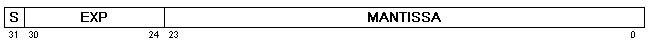
\includegraphics[]{c1.png} \\
        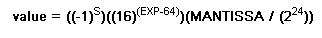
\includegraphics[]{c2.png} \\ 
    \end{center}
\end{figure}

Floating-point zero is represented by 32 bits of 0.

The IEEE format has 1 sign bit, $S$, an 8-bit offset (base 2) exponent
field, $E$, and a 24-bit mantissa, for which the high bit is (in normalized
numbers) always 1 and not part of the 23 bits in the format.

% insert image 3
\begin{figure}[!h]
    \begin{center}
        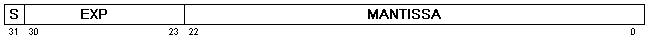
\includegraphics[]{c3.png} \\
    \end{center}
\end{figure}

If the exponent is not 255 and not 0, the value is a normalized floating point number,

% insert image 4
\begin{figure}[!h]
    \begin{center}
        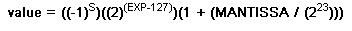
\includegraphics[]{c4.png} \\
    \end{center}
\end{figure}

If the exponent is 255 and the mantissa is 0, the value is plus or minus
infinity (depending on the sign bit).  If the exponent is 255 and the
mantissa is not 0, it indicates special values that will not be used in
this problem.

If the exponent is 0 and the mantissa is zero, the value is plus or
minus zero (depending on the sign bit).

If the exponent is 0 and the mantissa is not zero, the value is a
de-normalized floating-point number with:

% insert image 5
\begin{figure}[!h]
    \begin{center}
        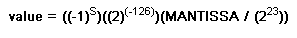
\includegraphics[]{c5.png} \\
    \end{center}
\end{figure}

Write a program that takes as input a floating-point value in Gould
format and outputs the value in IEEE format as follows:

If the value is zero return (plus) zero.

If the value is too large to be represented as a normalized floating-point
value, return plus or minus infinity depending on the sign.

If the value is too small to be represented as a normalized floating-point value:
\begin{itemize}
    \item If it may be represented as a de-normalized value, return the de-normalized value.
    \item Otherwise, return plus or minus zero, depending on the sign.
\end{itemize}

In all other cases, return the normalized value.

If there are less significant bits than required for IEEE floating-point, extend with 0 bits.

If there are more significant bits than required for IEEE floating-point, truncate the extra bits.

\section*{Input}

The first line of input contains a single integer $P$, 
($1 \le P \le 1000$) which is the number of data sets that follow.  
Each data set should be processed identically and independently.

Each data set consists of a single line of input.  It contains the
data set number, $K$, followed by 8 hex digits (\texttt{0-9,A-F}) of the Gould
floating-point value.


\section*{Output}

For each data set there is one line of output.  The single output line
consists of the data set number, $K$, followed by a single space followed
by the 8 hex digits (\texttt{0-9,A-F}) of the corresponding (as described above)
IEEE floating point value.


